\documentclass{beamer}
\usepackage[utf8]{inputenc}

\usetheme{Madrid}
\usecolortheme{default}
\usepackage{amsmath,amssymb,amsfonts,amsthm}
\usepackage{txfonts}
\usepackage{tkz-euclide}
\usepackage{listings}
\usepackage{adjustbox}
\usepackage{array}
\usepackage{tabularx}
\usepackage{gvv}
\usepackage{lmodern}
\usepackage{circuitikz}
\usepackage{tikz}
\usepackage{graphicx}

\setbeamertemplate{page number in head/foot}[totalframenumber]

\usepackage{tcolorbox}
\tcbuselibrary{minted,breakable,xparse,skins}



\definecolor{bg}{gray}{0.95}
\DeclareTCBListing{mintedbox}{O{}m!O{}}{%
  breakable=true,
  listing engine=minted,
  listing only,
  minted language=#2,
  minted style=default,
  minted options={%
    linenos,
    gobble=0,
    breaklines=true,
    breakafter=,,
    fontsize=\small,
    numbersep=8pt,
    #1},
  boxsep=0pt,
  left skip=0pt,
  right skip=0pt,
  left=25pt,
  right=0pt,
  top=3pt,
  bottom=3pt,
  arc=5pt,
  leftrule=0pt,
  rightrule=0pt,
  bottomrule=2pt,
  toprule=2pt,
  colback=bg,
  colframe=orange!70,
  enhanced,
  overlay={%
    \begin{tcbclipinterior}
    \fill[orange!20!white] (frame.south west) rectangle ([xshift=20pt]frame.north west);
    \end{tcbclipinterior}},
  #3,
}
\lstset{
    language=C,
    basicstyle=\ttfamily\small,
    keywordstyle=\color{blue},
    stringstyle=\color{orange},
    commentstyle=\color{green!60!black},
    numbers=left,
    numberstyle=\tiny\color{gray},
    breaklines=true,
    showstringspaces=false,
}
\begin{document}

\title 
{4.11.11}
\date{September 05,2025}


\author 
{Kavin B-EE25BTECH11033}






\frame{\titlepage}
\begin{frame}{Question}
Find the ratio in which the line $x - 3y = 0$ divides the line segment joining the points $(-2, -5)$ and $(6, 3)$. Find the coordinates of the point of intersection.\\
\end{frame}



\begin{frame}{Theoretical Solution}

Given the points,
\begin{align}
    \vec{A}=\begin{myvec}{-2\\-5}\end{myvec}\ \ 
    \vec{B}=\begin{myvec}{6\\3}\end{myvec}
\end{align}
\bigskip

Let the vector $\vec{P}$ be a point on the line $x - 3y = 0$ wihch divides the line segment joining the points $\vec{A}$ and $\vec{B}$.
\begin{align}
    \vec{P}=\begin{myvec}{3k\\k}\end{myvec} \;, 
\end{align}
The points $\vec{A}$, $\vec{P}$, $\vec{B}$ are collinear.\\
\end{frame}

\begin{frame}{Formulae}
\textbf{Points $\vec{A}, \vec{P}, \vec{B}$ are defined to be collinear if}
\begin{align}
		\rank{\myvec{\vec{P}-\vec{A}& \vec{B}-\vec{A}}} = 1
\end{align}
\end{frame}

\begin{frame}{Theoretical Solution}
\begin{align}
            \vec{P}-\vec{A} = \myvec{3k+2\\k+5}
\end{align}
\begin{align}
            \vec{B}-\vec{A} = \myvec{8\\8}
\end{align}
\begin{align}
            \myvec{\vec{P}-\vec{A}& \vec{B}-\vec{A}} = \myvec{3k+2 & 8\\k+5 & 8}
\end{align}
\begin{center}
$R_2 \rightarrow R_2 - \frac{k+5}{3k+2}R_1 \implies \myvec{3k+2 & 8\\0 & \frac{16k-24}{3k+2}}$
\end{center}
For rank $1$, the second row must be zero:
\begin{align}
    16k-24=0 \implies k=3/2
\end{align}
\begin{center}
$\therefore \vec{P}=\begin{myvec}{9/2\\3/2}\end{myvec}$
\end{center}
\end{frame}

\begin{frame}{Formulae}
\textbf{Section formula for a vector $\vec{P}$ which divides the line formed by vectors $\vec{A}$ and $\vec{B}$ in the ratio k:1 is given by}
\begin{align}
    \vec{P}=\frac{k\vec{B}+\vec{A}}{k+1}
\end{align}
\begin{align}
			k\brak{\vec{P}-\vec{B}}&= \vec{A}-\vec{P}
\end{align}
\begin{align}
			\implies k &=
			\frac{\brak{\vec{A}-\vec{P}}^{\top}\brak{\vec{P}-\vec{B}}}{\norm{\vec{P}-\vec{B}}^2}
			\label{eq:section_formula-k}
\end{align}
\end{frame}
\begin{frame}{Theoretical Solution}
\begin{align}
\brak{\vec{A}-\vec{P}}^{\top}\brak{\vec{P}-\vec{B}} = \myvec{-13/2 & -13/2}\myvec{-3/2\\-3/2} = 39/2\\
{\norm{\vec{P}-\vec{B}}^2} = \brak{\sqrt{\brak{-3/2}^2 + \brak{-3/2}^2}}^2 = 9/2
\end{align}

\begin{align}
\implies k &= 13/3
\end{align}

Therefore the ratio in which $\vec{P}$ divides the line segment joining the points $\vec{A}$ and $\vec{B}$ is $13:3$\\
\end{frame}


\begin{frame}{Plot}
    \centering
    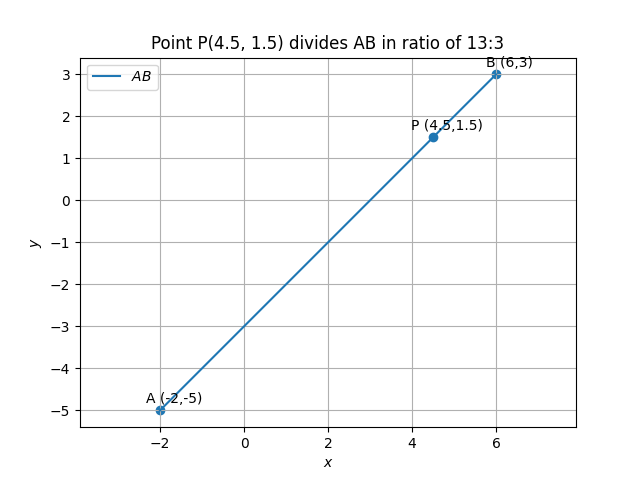
\includegraphics[width=\columnwidth, height=0.8\textheight, keepaspectratio]{figs/fig.png}     
\end{frame}


\end{document}
